\documentclass[11pt,a4paper]{article}

% ---------- packages ----------
\usepackage[margin=2.4cm]{geometry}
\usepackage{times}
\usepackage{amsmath,amssymb,amsfonts}
\usepackage{booktabs}
\usepackage{tabularx}
\usepackage{multirow}
\usepackage{graphicx}
\usepackage{subcaption}
\usepackage{float}
\usepackage{xcolor}
\usepackage{hyperref}
\usepackage{enumitem}
\usepackage{setspace}
\usepackage{microtype}
\usepackage{caption}
\usepackage{array}
\usepackage{makecell}

\hypersetup{
  colorlinks=true,
  linkcolor=black,
  citecolor=black,
  urlcolor=blue
}

\captionsetup{font=small,labelfont=bf}
\onehalfspacing
\graphicspath{{figures/}}

\title{
\vspace{-1.2em}
\textbf{An Empirical Reproduction and Extension of Auditory Filter Model Frontends for Speaker Gender Recognition}\\[0.6em]
\large Implementation Report --- Code Aligned with SGR\_AFM + Novel Reduced Variants
}
\author{
  Reproduction of Fayyazi \& Shekofteh (2023)\\[0.3em]
  \normalsize\textit{Applied Acoustics}, Vol.~213, Art.~109635
}
\date{1405/07/11 (2026-10-03)}

\begin{document}
\maketitle

\begin{abstract}
\noindent
This report presents an end-to-end reproduction of the auditory filter model (AFM) convolutional frontend framework for binary speaker gender recognition proposed by Fayyazi and Shekofteh (2023), with kernels, cutoffs, LayerNorm, optimizer, and evaluation protocol aligned to the authors' public SGR\_AFM code. We train Free-CNN, Mel-CNN, Sinc, Sinc2, Gamma, Gauss, Cascade, and a Mean-shift Reduced bank on TIMIT (50 epochs), fine-tune on LibriSpeech \texttt{dev-clean} (20 epochs), and evaluate on RAVDESS and VoxCeleb1-test. On TIMIT, Cascade reaches \textbf{99.18\%} accuracy (paper 99.16\%). The best transfer AFM is Sinc on VoxCeleb1-test (\textbf{96.96\%}). We further propose two Reduced-bank alternatives at equal filter count $K{=}43$: \emph{task-aware ERB clustering} (frozen sinc$^2$, cross-entropy) and \emph{task-aware distilled} (same filter selection with knowledge distillation from Cascade and trainable cutoffs). \textbf{Task-aware distilled} improves RAVDESS accuracy by \textbf{+6.05} and VoxCeleb1-test by \textbf{+1.95} percentage points over the paper Mean-shift Reduced baseline under identical training budgets.
\end{abstract}

\tableofcontents
\newpage

% ============================================================
\section{Introduction}
% ============================================================

Speaker gender recognition (SGR) classifies a talker as male or female from the acoustic signal. Deep networks on raw waveforms can be accurate, but unconstrained first-layer filters are hard to interpret. Fayyazi and Shekofteh~\cite{fayyazi2023} replace free kernels with parametric \emph{auditory filter models} (AFMs)---Sinc, Sinc2, Gammatone, Gaussian, Cascaded Gaussian---and prune Cascade poles with mean-shift to form a compact Reduced bank.

This work:
\begin{enumerate}[leftmargin=1.6em,itemsep=0.25em]
  \item reproduces the SGR\_AFM architecture and training protocol as faithfully as available data and compute allow;
  \item reports CER, FER, and utterance accuracy on TIMIT, RAVDESS, and VoxCeleb1-test;
  \item analyzes discrepancies with published Tables~4, 7 and~8;
  \item introduces task-aware ERB clustering and task-aware distilled Reduced models at fixed filter count $K$.
\end{enumerate}

% ============================================================
\section{Method Overview}
% ============================================================

\subsection{Task definition and metrics}

Given waveform $x$, predict $y\in\{0,1\}$ (male/female). Chunks of $T{=}200$\,ms with hop $H{=}10$\,ms are used at evaluation. Following the authors' evaluation protocol, the utterance decision is the argmax of \emph{summed} chunk log-probabilities (not majority vote). We report:
\begin{itemize}[leftmargin=1.6em,itemsep=0.2em]
  \item \textbf{FER:} mean per-utterance frame error;
  \item \textbf{CER:} utterance error after summed-logp decision;
  \item \textbf{Accuracy:} $100-\mathrm{CER}$ (\%).
\end{itemize}

\subsection{Network architecture}

The backbone matches the authors' SGR\_AFM network:
\begin{align*}
  x &\xrightarrow{\;\mathrm{LN}\;} \mathrm{Conv1}\to \lvert\cdot\rvert \to \mathrm{Pool}_3 \to \mathrm{LN} \to \mathrm{LReLU}\\
    &\xrightarrow{\;\mathrm{Conv2}\;} \mathrm{Pool}_3 \to \mathrm{LN} \to \mathrm{LReLU}\\
    &\xrightarrow{\;\mathrm{Conv3}\;} \mathrm{Pool}_3 \to \mathrm{LN} \to \mathrm{LReLU}\\
    &\to \mathrm{Flatten} \to \mathrm{LN} \to (\mathrm{FC}_{2048}+\mathrm{BN}_{0.05})\times 3 \to \mathrm{Softmax}_2.
\end{align*}
Conv1 uses $N{=}80$ filters of length $L{=}257$ (Reduced: $N{=}K{=}43$). Conv2/Conv3: 60 filters, kernel 5. Loss: cross-entropy. Optimizer: RMSprop, $\mathrm{lr}{=}10^{-3}$, $\alpha{=}0.95$, $\varepsilon{=}10^{-8}$, batch 128.

\subsection{Auditory filter model frontends}

Learned cutoffs follow the authors: $\mathrm{norm\_f1}=f_1/f_s$, $\mathrm{norm\_f2}=f_2/f_s$, with
\[
f_1=\lvert nf_1\rvert+\tfrac{50}{f_s},\qquad
f_2=f_1+\lvert nf_2-f_1\rvert+\tfrac{50}{f_s}.
\]
Kernels (sinc, sinc2, gamma, gauss, cascade) match the authors' public SGR\_AFM implementation.

\begin{table}[H]
\centering
\caption{First-layer frontends considered in this study.}
\label{tab:frontends}
\begin{tabular}{@{}llp{7.2cm}@{}}
\toprule
\textbf{Name} & \textbf{Type} & \textbf{Description} \\
\midrule
Free-CNN & Unconstrained & Fully learnable FIR kernels \\
Mel-CNN  & Fixed         & Frozen Mel-scaled filter bank \\
Sinc     & AFM           & Band-pass sinc \\
Sinc2    & AFM           & Squared-sinc / triangular spectrum \\
Gamma    & AFM           & Gammatone impulse response \\
Gauss    & AFM           & Gaussian band-pass \\
Cascade  & AFM           & Cascade of two Gaussians (two poles/filter) \\
Reduced  & Pruned        & Mean-shift of Cascade poles $\to$ frozen sinc$^2$ bank \\
\bottomrule
\end{tabular}
\end{table}

\subsection{Paper pole reduction (Reduced model)}

Cascade stages yield 160 bands $(f_1,f_2)$, mapped to poles
\begin{equation}
  x = e^{-\sigma + j\omega_0},\quad
  \omega_0=\frac{2\pi(f_1+f_2)}{2f_s},\quad
  \sigma=\frac{2\pi(f_2-f_1)}{f_s}.
\end{equation}
MeanShift with bandwidth $0.079$ clusters $(\mathrm{Re}\,x,\mathrm{Im}\,x)$. Cluster-mean cutoffs initialize a \textbf{frozen} sinc$^2$ bank. In this run: \textbf{160 poles $\to$ 43 filters}.

% ============================================================
\section{Experimental Pipeline}
% ============================================================

\begin{enumerate}[leftmargin=1.6em,itemsep=0.35em]
  \item \textbf{Preprocessing.} TIMIT: peak-normalize and trim to word boundaries; LibriSpeech: remove silences $\ge 1$\,s below $-30$\,dB; RAVDESS/Vox: raw.
  \item \textbf{TIMIT training.} Free, Mel, Sinc, Sinc2, Gamma, Gauss, Cascade --- 50 epochs.
  \item \textbf{Paper Reduced.} Mean-shift $\to$ 43 frozen sinc$^2$ $\to$ 50 epochs TIMIT.
  \item \textbf{Fine-tuning.} 20 epochs on LibriSpeech \texttt{dev-clean}; eval RAVDESS and VoxCeleb1-test (Mel skipped, as in paper Tables~7--8).
  \item \textbf{Analyses.} Accumulative magnitude, $f_c$ histogram, $Q$, $f_1/f_2$, t-SNE, pole plane.
  \item \textbf{Innovation.} Task-aware ERB and task-aware distilled Reduced models at $K{=}43$.
\end{enumerate}

% ============================================================
\section{Training Configuration}
% ============================================================

\begin{table}[H]
\centering
\caption{Learning settings: paper vs.\ this work.}
\label{tab:hparams}
\begin{tabular}{@{}lll@{}}
\toprule
\textbf{Parameter} & \textbf{Paper} & \textbf{This work} \\
\midrule
Input                 & Raw waveform, 16\,kHz          & Identical \\
Chunk / hop           & 200\,ms / 10\,ms               & Eval: identical; train: 8 random chunks/utt/epoch \\
Gain augmentation     & Random amplitude               & Uniform in $[0.8,1.2]$ \\
Conv1                 & 80$\times$257                  & Identical (Reduced: 43) \\
Conv2 / Conv3         & 60, kernel 5, pool 3           & Identical \\
Classifier            & $3\times$FC\,2048 + BN         & Identical (BN momentum 0.05) \\
Loss / optimizer      & NLL / RMSprop, $\mathrm{lr}{=}10^{-3}$ & Identical \\
Batch size            & 128                            & 128 \\
TIMIT epochs          & 500                            & \textbf{50} \\
Fine-tune epochs      & 200 on \texttt{train-clean-360}& \textbf{20} on \texttt{dev-clean} \\
Independent runs      & 3 (mean $\pm$ std)             & \textbf{1} (seed 42) \\
VoxCeleb evaluation   & Broader VoxCeleb1 setup        & VoxCeleb1-test (4874 utt.) \\
\bottomrule
\end{tabular}
\end{table}

\paragraph{Data note.}
TIMIT split matches the paper (2960 / 736 / 1344). Gender is \emph{not} balanced ($\sim$70\% male), as in~\cite{fayyazi2023}. Fine-tuning uses \texttt{dev-clean} because \texttt{train-clean-360} was unavailable.

% ============================================================
\section{Results: Paper Reproduction}
% ============================================================

\subsection{TIMIT (in-domain)}
\label{sec:timit}

\begin{table}[H]
\centering
\caption{TIMIT full test set: paper (mean of 3 runs) vs.\ this work (1 run). $\Delta=$ Ours $-$ Paper.}
\label{tab:timit}
\small
\begin{tabular}{@{}lrrrrrrr@{}}
\toprule
\textbf{Method} & \textbf{P.Acc} & \textbf{O.Acc} & $\boldsymbol{\Delta}$ & \textbf{P.CER} & \textbf{O.CER} & \textbf{P.FER} & \textbf{O.FER} \\
\midrule
Free-CNN & 98.84 & 98.66 & $-0.18$ & 1.16 & 1.34 & 3.14 & 3.88 \\
Mel-CNN  & 98.64 & 98.66 & $+0.02$ & 1.36 & 1.34 & 4.92 & 3.52 \\
Sinc     & 98.84 & 98.88 & $+0.04$ & 1.16 & 1.12 & 2.93 & 3.29 \\
Sinc2    & 99.03 & 98.88 & $-0.15$ & 0.97 & 1.12 & 3.16 & 3.72 \\
Gamma    & 99.01 & 98.88 & $-0.13$ & 0.99 & 1.12 & 2.96 & 3.25 \\
Gauss    & 98.91 & 98.88 & $-0.03$ & 1.09 & 1.12 & 2.90 & 3.09 \\
Cascade  & \textbf{99.16} & \textbf{99.18} & $\boldsymbol{+0.02}$ & \textbf{0.84} & \textbf{0.82} & \textbf{2.88} & 3.06 \\
Reduced  & 99.03 & 98.07 & $-0.96$ & 0.97 & 1.93 & 3.94 & 5.99 \\
\bottomrule
\end{tabular}
\end{table}

\begin{figure}[H]
\centering
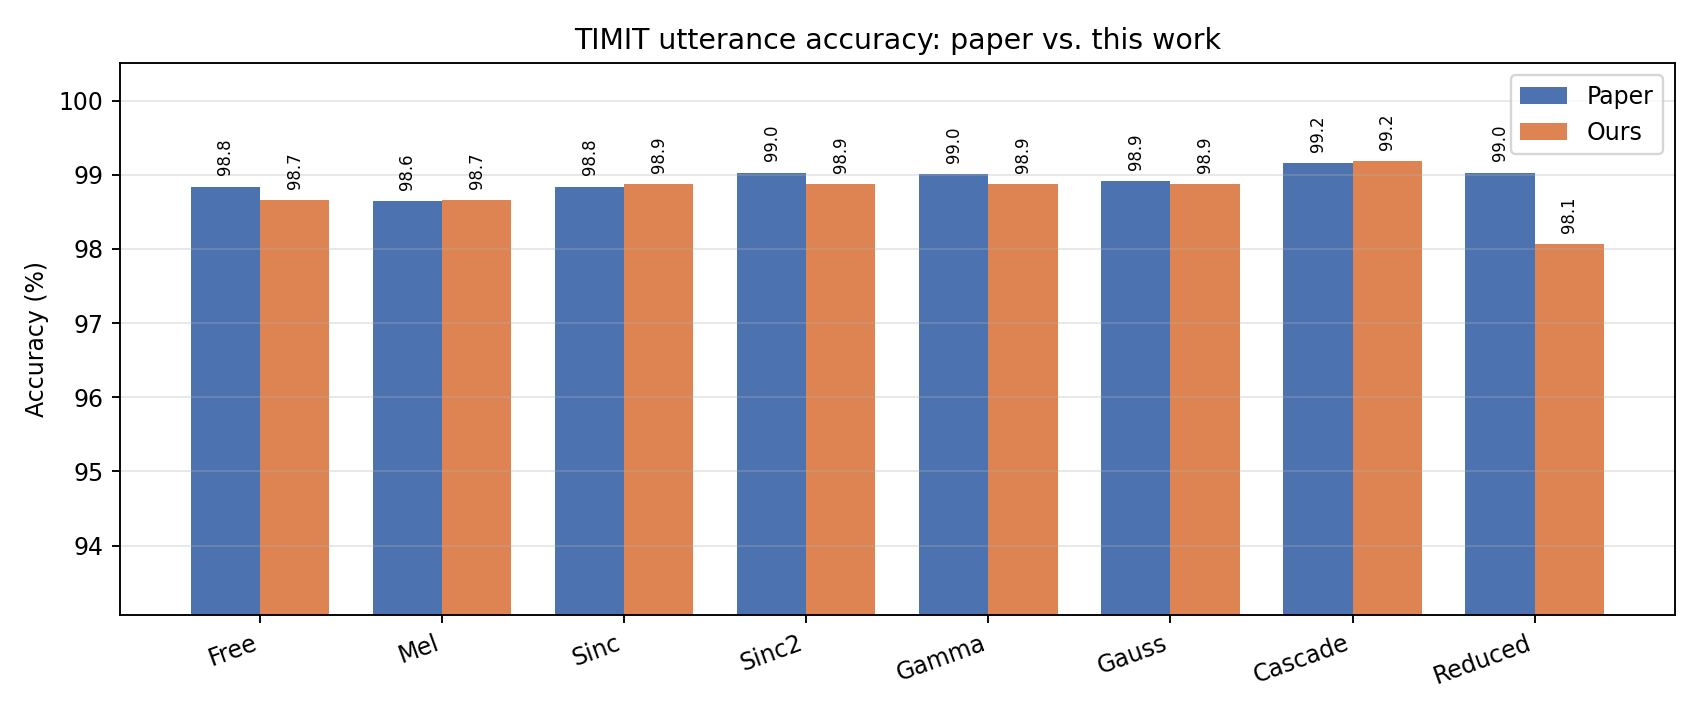
\includegraphics[width=0.92\textwidth]{bar_timit_acc.png}
\caption{TIMIT utterance accuracy: paper mean vs.\ this work.}
\label{fig:bar-timit}
\end{figure}

Cascade essentially matches the paper. Other AFMs lie within $\sim$0.2\,pp. Paper-style Reduced ($K{=}43$, frozen) trails the published Reduced mean under the shorter 50-epoch retrain.

\subsection{LibriSpeech fine-tuning}
\label{sec:libri-ft}

After TIMIT training, each frontend except Mel is fine-tuned for \textbf{20 epochs} on LibriSpeech \texttt{dev-clean} (RMSprop, batch 128, same chunking as training). Utterance decisions use summed chunk log-probabilities. Table~\ref{tab:libri-ft} reports training-split accuracy at the final epoch and validation-monitor accuracy / CER / FER at the best-validation epoch (speaker-held-out subset of \texttt{dev-clean}). These are \emph{adaptation} metrics; RAVDESS and VoxCeleb1-test below are the paper-style generalization tests after this stage.

\begin{table}[H]
\centering
\caption{LibriSpeech fine-tuning (20 epochs on \texttt{dev-clean}). Train = final-epoch utterance accuracy on the fine-tune training split; Val = best epoch on the validation monitor.}
\label{tab:libri-ft}
\small
\begin{tabular}{@{}lrrrrr@{}}
\toprule
\textbf{Method} & \textbf{Train Acc} & \textbf{Val Acc} & \textbf{Val CER} & \textbf{Val FER} \\
\midrule
Free-CNN & 94.74 & 89.46 & 10.54 & 21.53 \\
Sinc     & 92.08 & 89.46 & 10.54 & 18.74 \\
Sinc2    & 91.93 & 89.46 & 10.54 & 21.86 \\
Gamma    & 92.75 & 89.46 & 10.54 & 19.44 \\
Gauss    & 92.36 & \textbf{89.59} & \textbf{10.41} & 19.72 \\
Cascade  & 92.92 & 89.46 & 10.54 & 19.67 \\
Reduced  & 87.22 & 89.46 & 10.54 & 22.91 \\
\bottomrule
\end{tabular}
\end{table}

\begin{figure}[H]
\centering
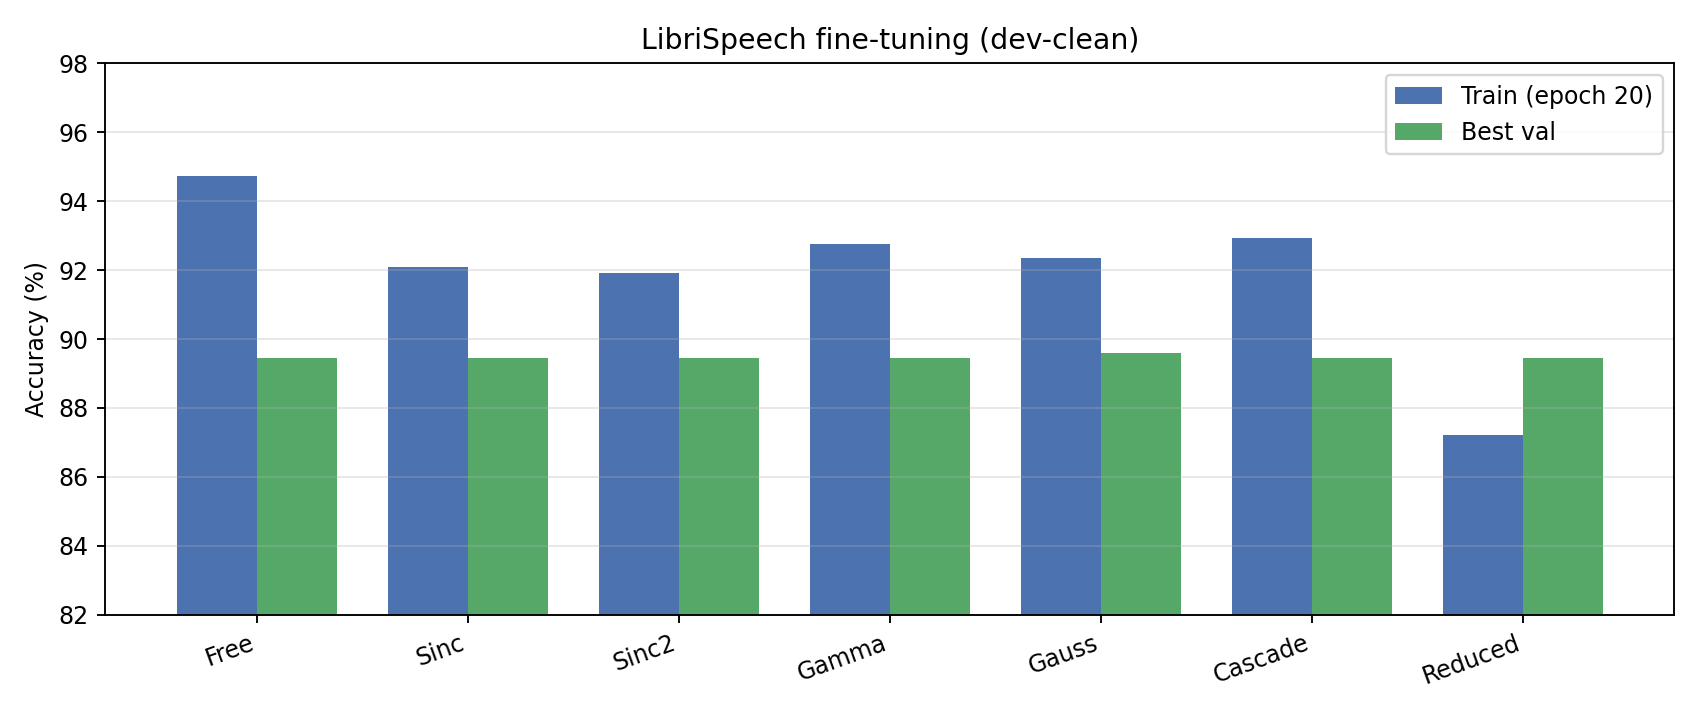
\includegraphics[width=0.88\textwidth]{bar_librispeech_ft.png}
\caption{LibriSpeech fine-tuning: final training accuracy vs.\ best validation accuracy (\%).}
\label{fig:bar-libri-ft}
\end{figure}

Validation accuracy is similar across frontends ($\sim$89.5\%), while final training accuracy varies more (e.g., Free-CNN fits the adaptation set fastest; Reduced lags on the training split but still reaches comparable validation Acc).

\subsection{RAVDESS after fine-tuning}
\label{sec:ravdess}

\begin{table}[H]
\centering
\caption{RAVDESS after LibriSpeech fine-tuning. Paper: published Table~8 (accuracy only). Ours: full test set (1440 utt.). $\Delta=$ Ours $-$ Paper (Acc).}
\label{tab:ravdess}
\small
\begin{tabular}{@{}lrrrrrrr@{}}
\toprule
\textbf{Method} & \textbf{P.Acc} & \textbf{O.Acc} & $\boldsymbol{\Delta}$ & \textbf{O.CER} & \textbf{O.FER} \\
\midrule
Free-CNN & 93.54 & 88.47 & $-5.07$ & 11.53 & 26.17 \\
Sinc     & 96.32 & 94.65 & $-1.67$ & 5.35 & 25.41 \\
Sinc2    & 94.86 & 93.47 & $-1.39$ & 6.53 & 28.06 \\
Gamma    & 97.78 & 96.04 & $-1.74$ & 3.96 & 27.53 \\
Gauss    & 93.19 & \textbf{95.21} & $\boldsymbol{+2.02}$ & 4.79 & 27.51 \\
Cascade  & \textbf{97.99} & 95.49 & $-2.50$ & 4.51 & 26.32 \\
Reduced  & 96.11 & 89.58 & $-6.53$ & 10.42 & 28.88 \\
\bottomrule
\end{tabular}
\end{table}

\begin{figure}[H]
\centering
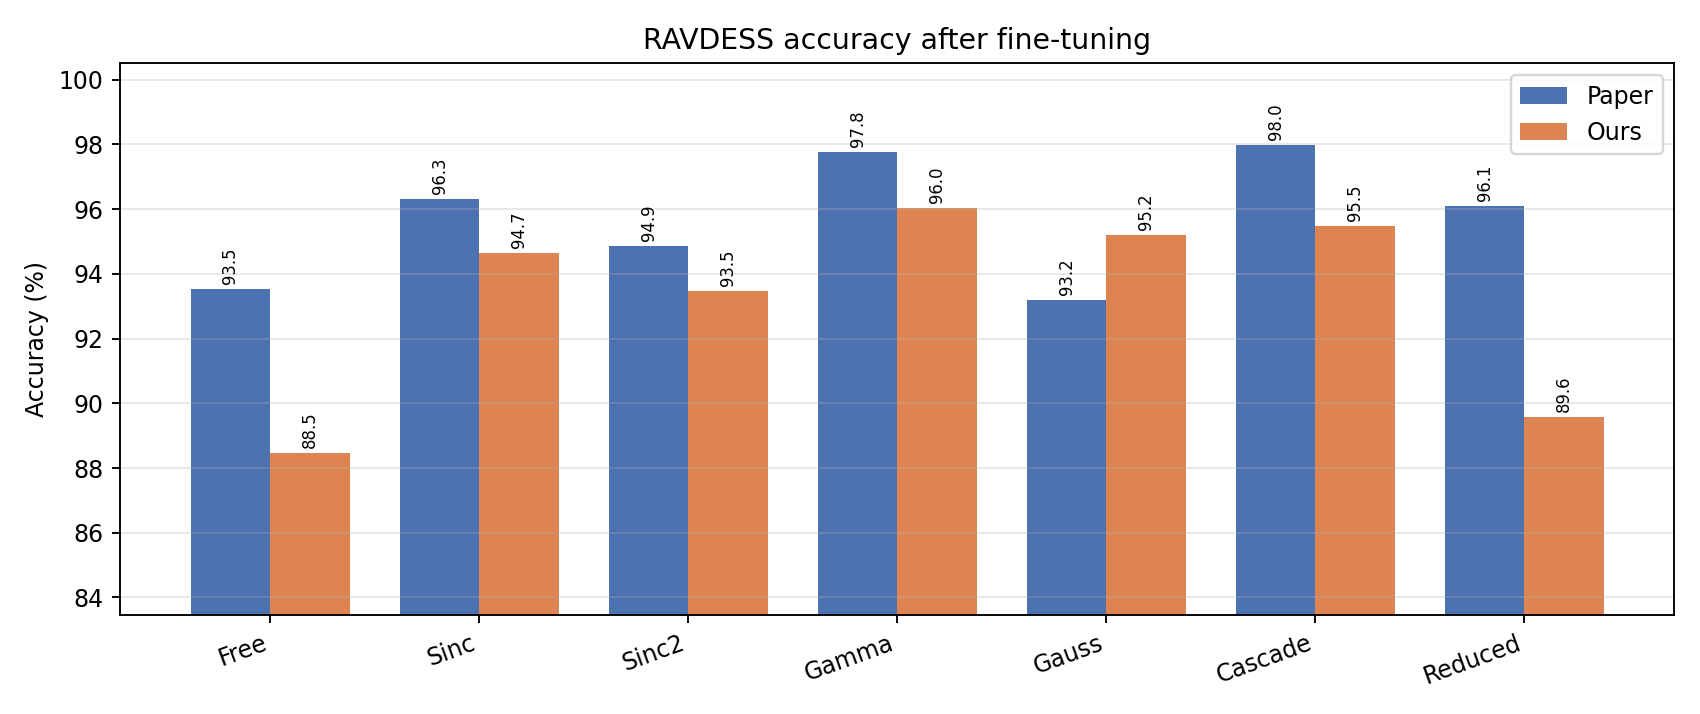
\includegraphics[width=0.92\textwidth]{bar_ravdess_acc.png}
\caption{RAVDESS accuracy after fine-tuning: paper vs.\ this work.}
\label{fig:bar-rav}
\end{figure}

\subsection{VoxCeleb1-test after fine-tuning}
\label{sec:vox}

\begin{table}[H]
\centering
\caption{VoxCeleb1-test after LibriSpeech fine-tuning. Paper: published Table~7 (full VoxCeleb1; accuracy only). Ours: VoxCeleb1-test (4874 utt.). $\Delta=$ Ours $-$ Paper (Acc).}
\label{tab:vox}
\small
\begin{tabular}{@{}lrrrrrrr@{}}
\toprule
\textbf{Method} & \textbf{P.Acc} & \textbf{O.Acc} & $\boldsymbol{\Delta}$ & \textbf{O.CER} & \textbf{O.FER} \\
\midrule
Free-CNN & 97.48 & 76.16 & $-21.32$ & 23.84 & 31.45 \\
Sinc     & \textbf{97.66} & \textbf{96.96} & $-0.70$ & 3.04 & 17.30 \\
Sinc2    & 96.33 & 95.38 & $-0.95$ & 4.62 & 17.87 \\
Gamma    & 97.17 & 95.88 & $-1.29$ & 4.12 & 18.65 \\
Gauss    & 96.74 & 95.69 & $-1.05$ & 4.31 & 17.69 \\
Cascade  & 97.27 & 96.80 & $-0.47$ & 3.20 & 17.44 \\
Reduced  & 97.44 & 91.53 & $-5.91$ & 8.47 & 23.17 \\
\bottomrule
\end{tabular}
\end{table}

\begin{figure}[H]
\centering
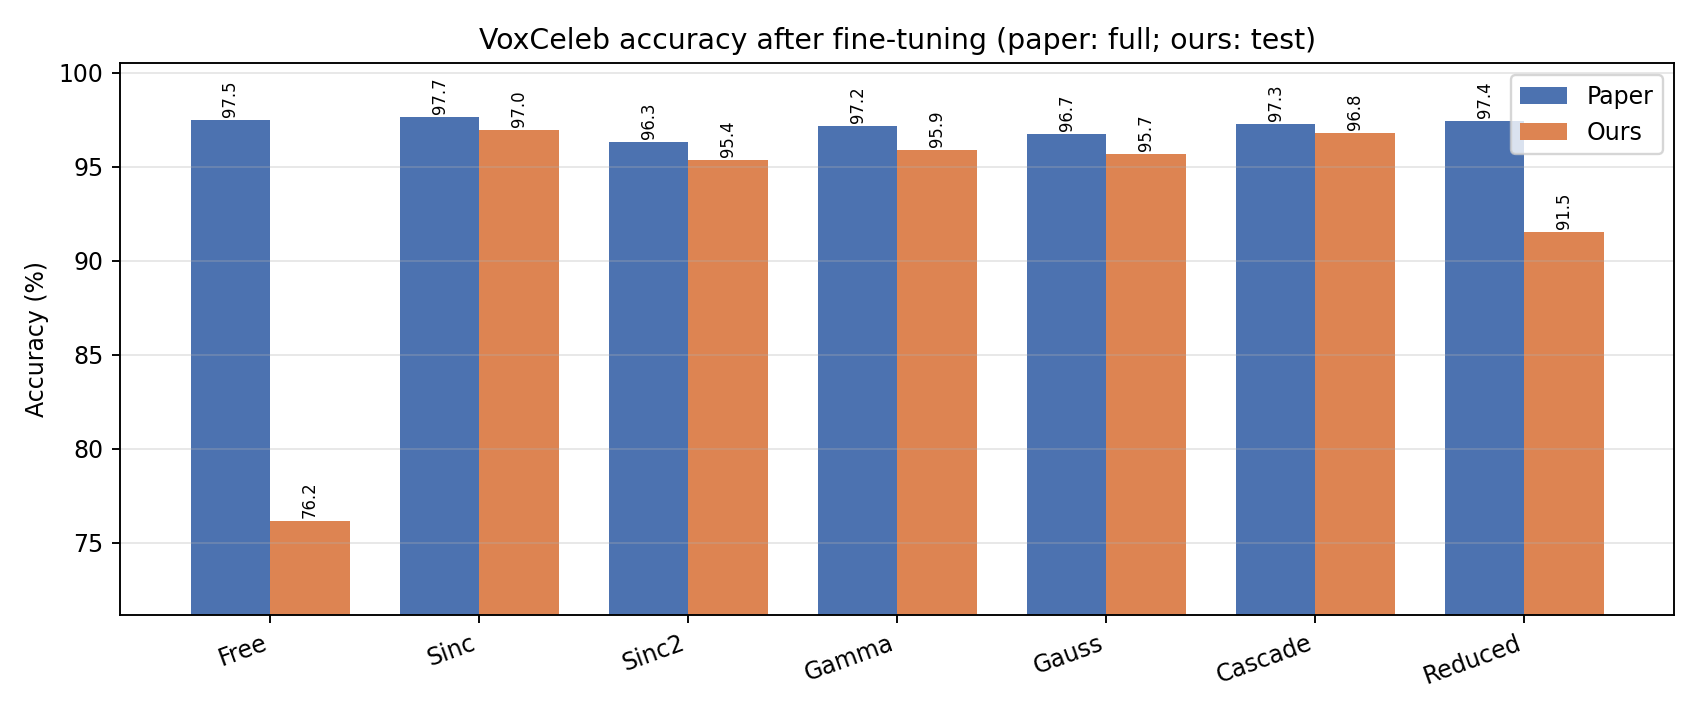
\includegraphics[width=0.92\textwidth]{bar_vox_acc.png}
\caption{VoxCeleb accuracy after fine-tuning: paper vs.\ this work (test).}
\label{fig:bar-vox}
\end{figure}

Sinc is the strongest transfer model here (within 0.7\,pp of the paper). Free-CNN collapses on Vox under the short / small fine-tune. Cascade stays within 0.5\,pp on this split.

% ============================================================
\section{Training Dynamics}
\label{sec:curves}
% ============================================================

\begin{figure}[H]
\centering
\begin{subfigure}[t]{0.48\textwidth}
  \centering
  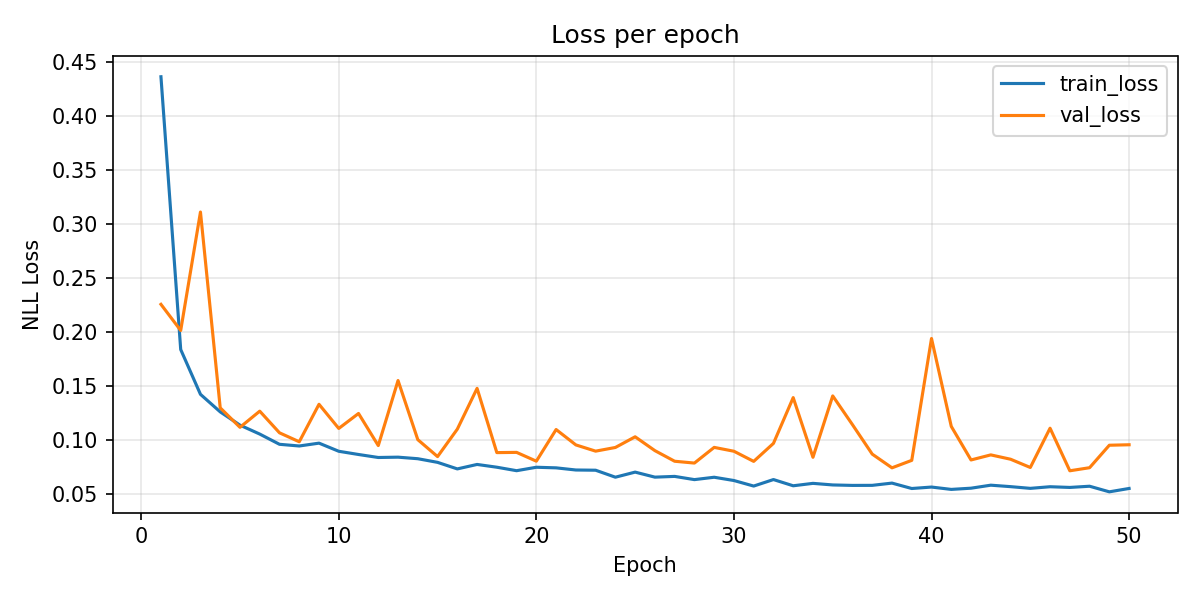
\includegraphics[width=\linewidth]{cascade_timit_loss.png}
  \caption{Loss}
\end{subfigure}\hfill
\begin{subfigure}[t]{0.48\textwidth}
  \centering
  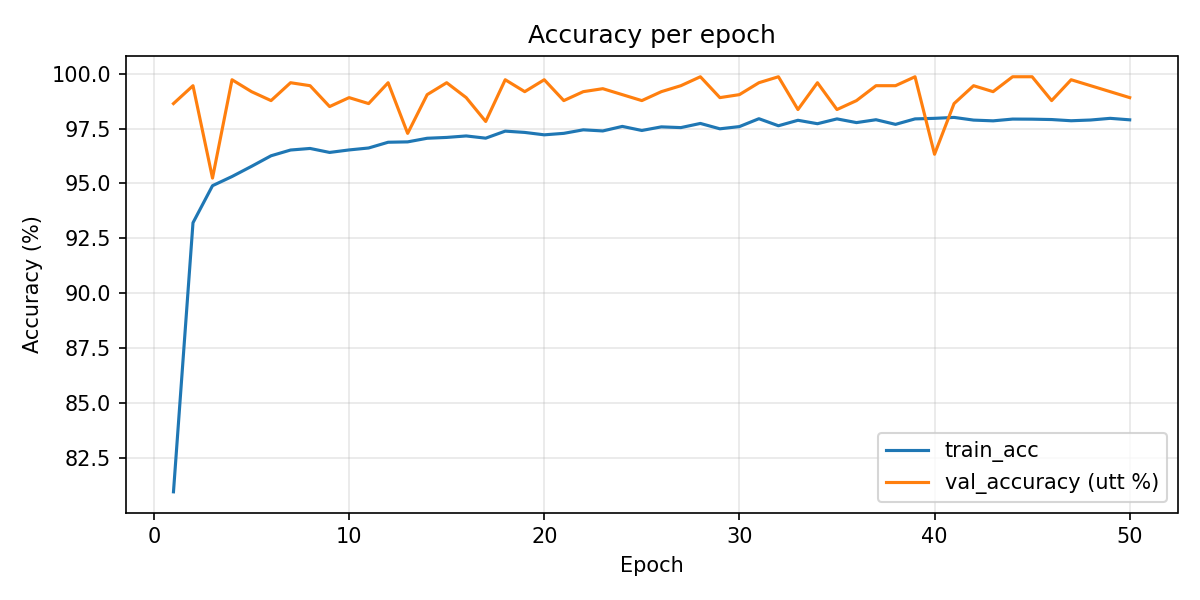
\includegraphics[width=\linewidth]{cascade_timit_acc.png}
  \caption{Accuracy}
\end{subfigure}
\caption{Cascade --- TIMIT training (50 epochs).}
\label{fig:cascade-timit-curves}
\end{figure}

\begin{figure}[H]
\centering
\begin{subfigure}[t]{0.48\textwidth}
  \centering
  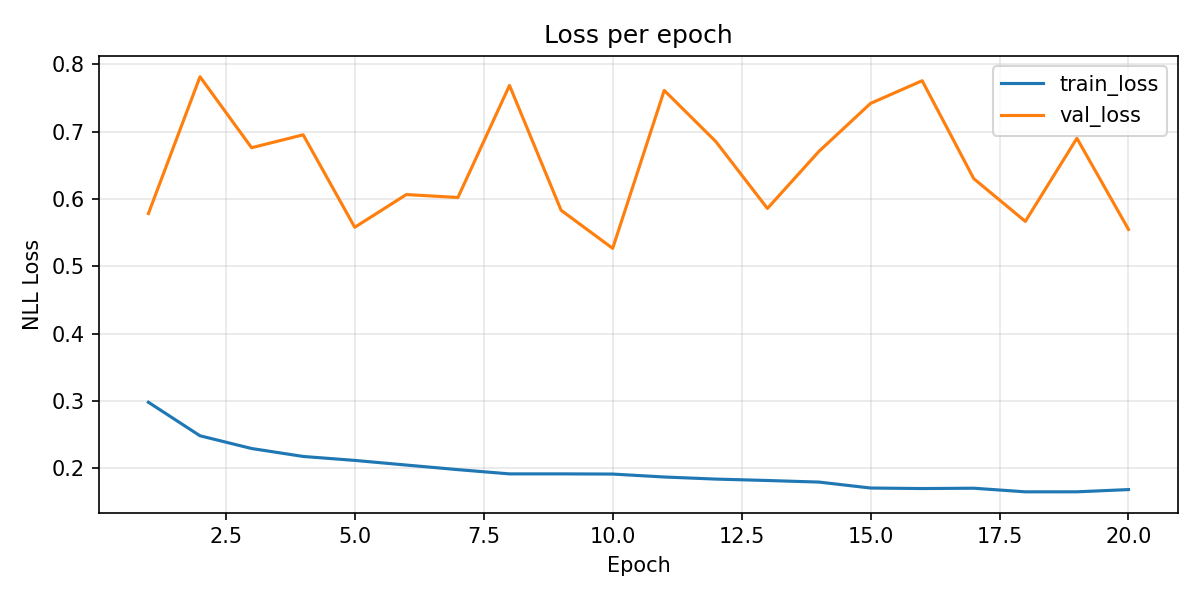
\includegraphics[width=\linewidth]{cascade_ft_loss.png}
  \caption{Loss}
\end{subfigure}\hfill
\begin{subfigure}[t]{0.48\textwidth}
  \centering
  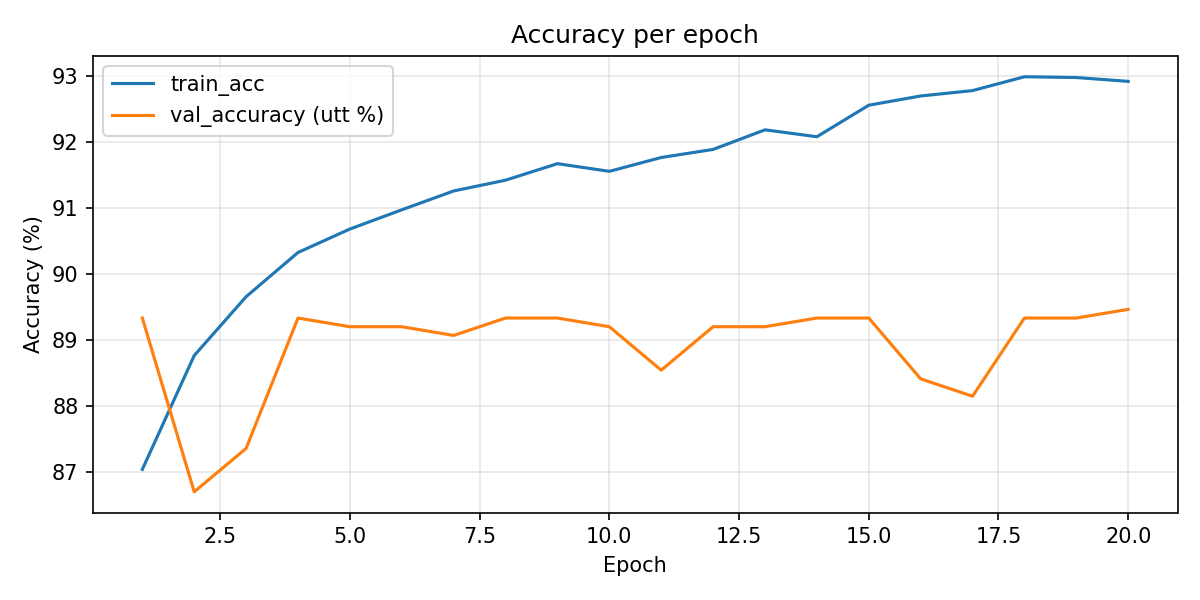
\includegraphics[width=\linewidth]{cascade_ft_acc.png}
  \caption{Accuracy}
\end{subfigure}
\caption{Cascade --- LibriSpeech fine-tuning (20 epochs).}
\label{fig:cascade-ft-curves}
\end{figure}

\begin{figure}[H]
\centering
\begin{subfigure}[t]{0.48\textwidth}
  \centering
  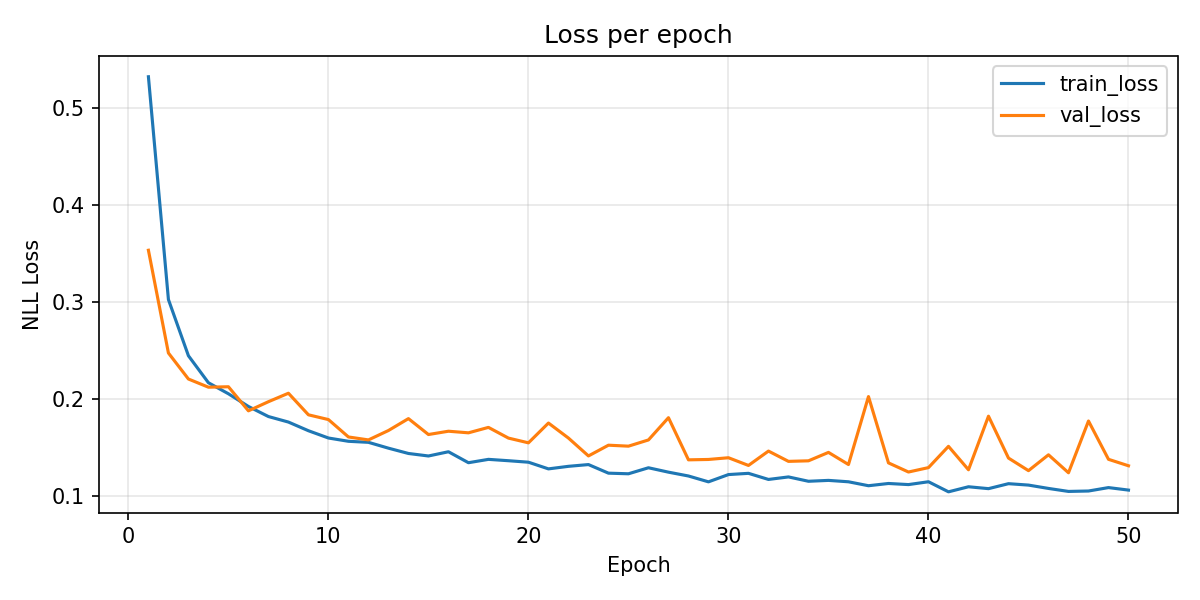
\includegraphics[width=\linewidth]{reduced_timit_loss.png}
  \caption{Loss}
\end{subfigure}\hfill
\begin{subfigure}[t]{0.48\textwidth}
  \centering
  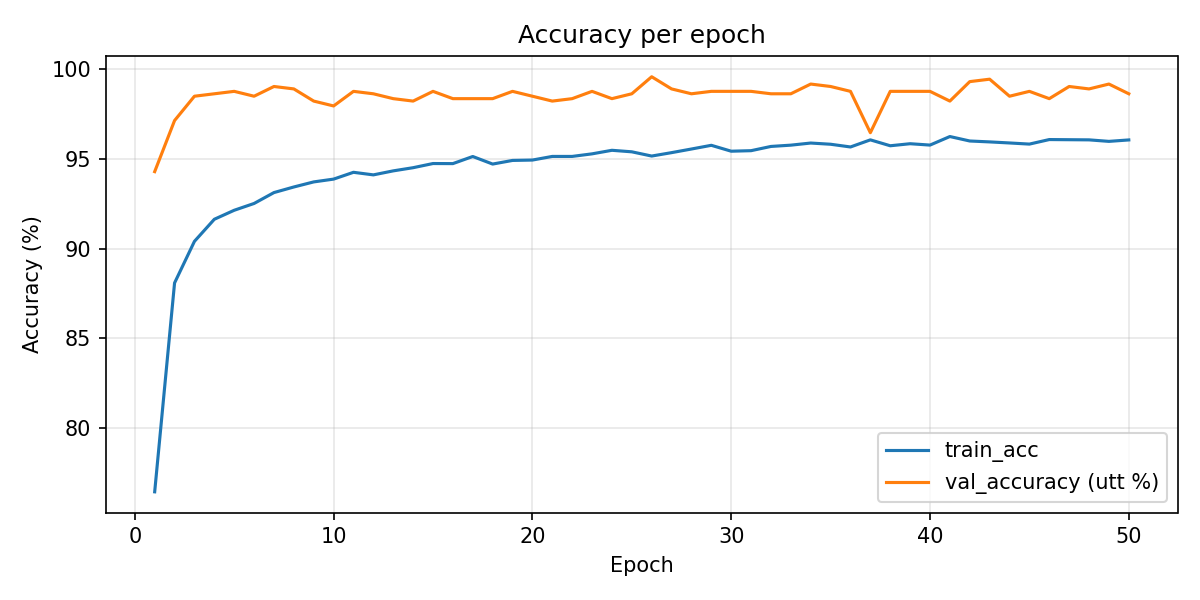
\includegraphics[width=\linewidth]{reduced_timit_acc.png}
  \caption{Accuracy}
\end{subfigure}
\caption{Paper Reduced --- TIMIT retraining after Mean-shift pruning (50 epochs, frozen Conv1).}
\label{fig:reduced-timit-curves}
\end{figure}

\begin{figure}[H]
\centering
\begin{subfigure}[t]{0.48\textwidth}
  \centering
  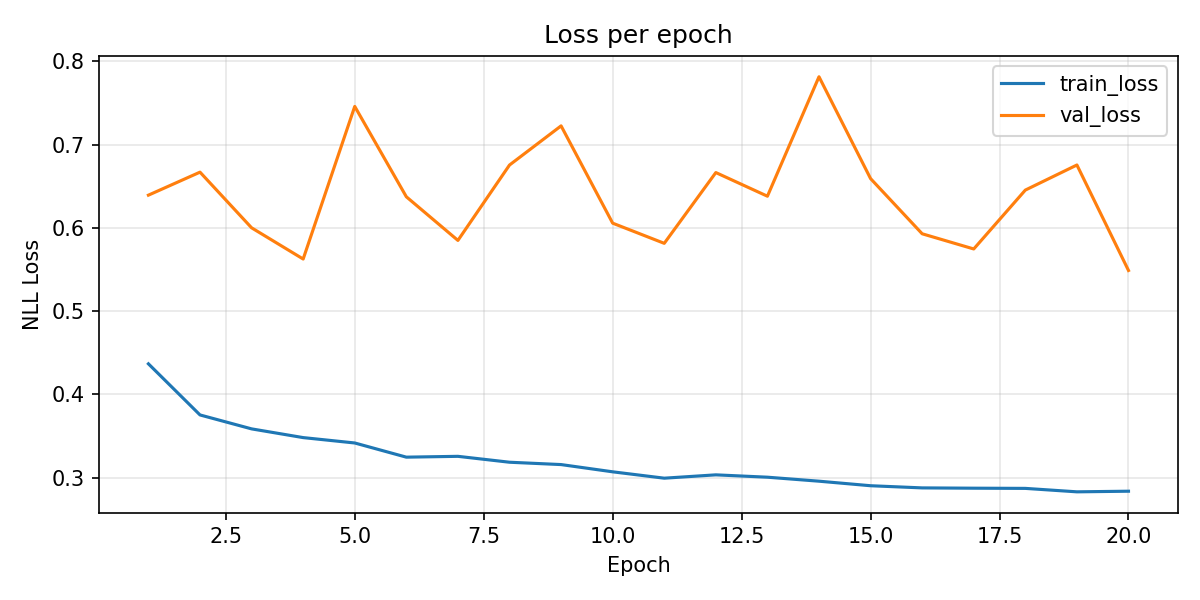
\includegraphics[width=\linewidth]{reduced_ft_loss.png}
  \caption{Loss}
\end{subfigure}\hfill
\begin{subfigure}[t]{0.48\textwidth}
  \centering
  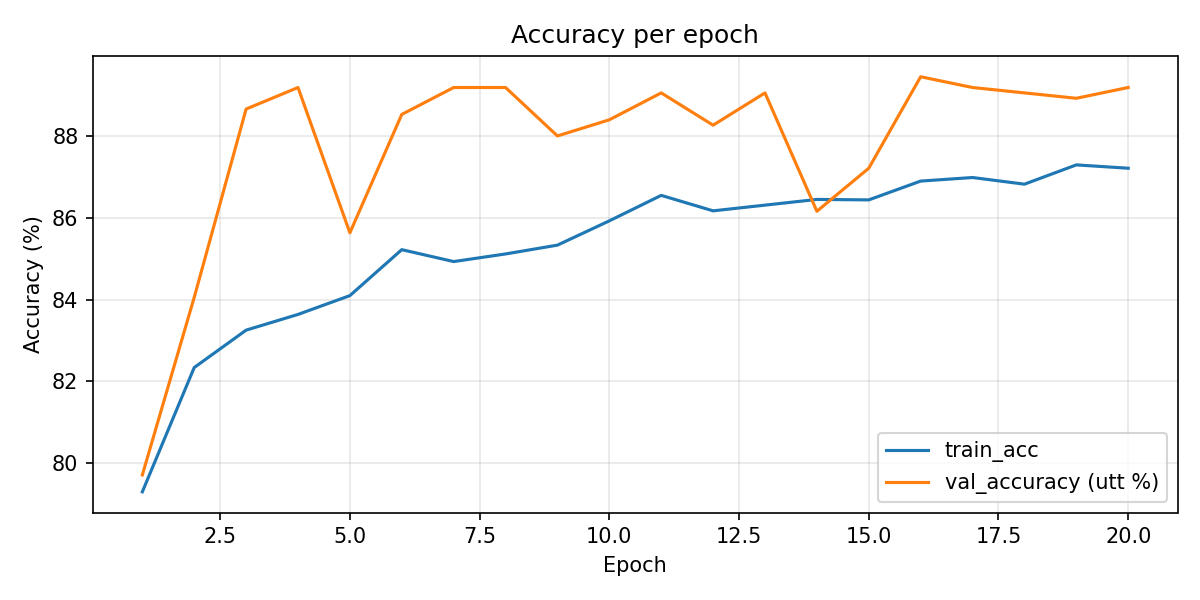
\includegraphics[width=\linewidth]{reduced_ft_acc.png}
  \caption{Accuracy}
\end{subfigure}
\caption{Paper Reduced --- LibriSpeech fine-tuning (20 epochs).}
\label{fig:reduced-ft-curves}
\end{figure}

% ============================================================
\section{Pole Reduction on the Complex Plane}
\label{sec:poles}
% ============================================================

\begin{figure}[H]
\centering
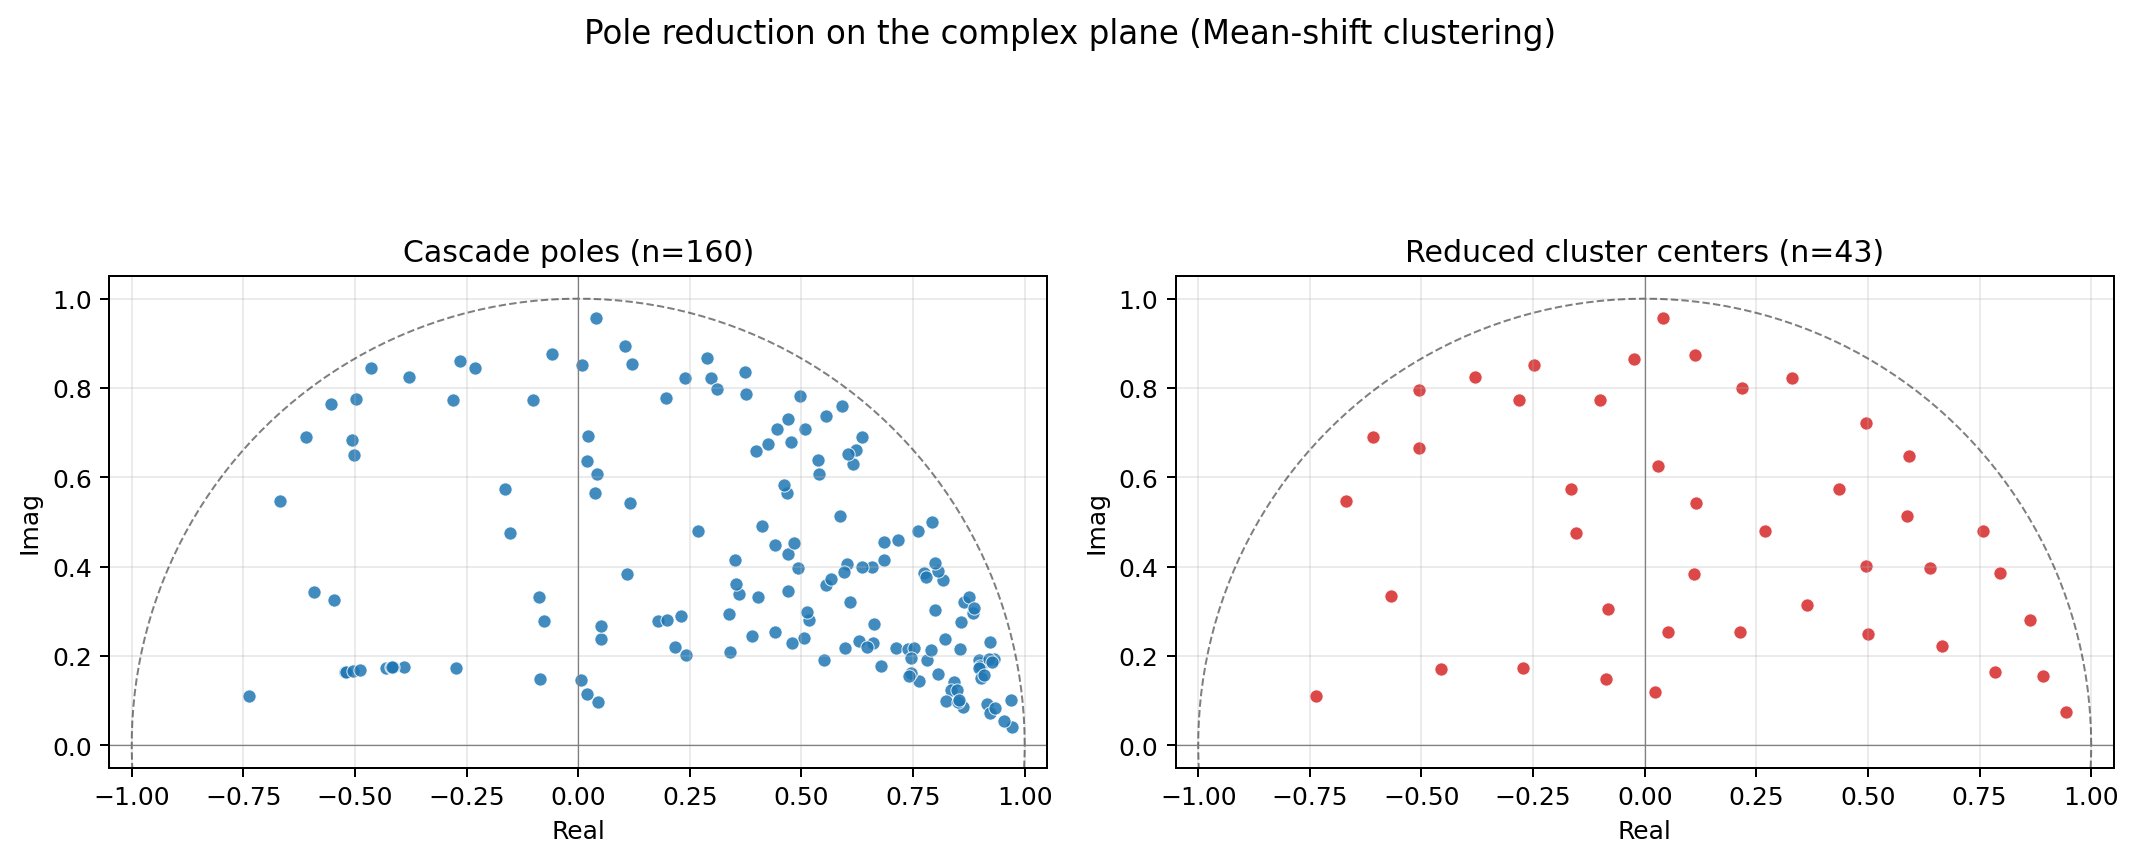
\includegraphics[width=0.98\textwidth]{pole_reduction.png}
\caption{Pole reduction on the complex plane. Left: 160 Cascade poles. Right: Mean-shift centers ($K{=}43$) used by the paper Reduced frontend.}
\label{fig:poles}
\end{figure}

Angle encodes center frequency; distance from the unit circle relates to bandwidth. Clustering with bandwidth $0.079$ merges nearby poles into 43 representatives.

% ============================================================
\section{Filter Interpretability Analysis}
\label{sec:analysis}
% ============================================================

\begin{figure}[H]
\centering
\begin{subfigure}[t]{0.48\textwidth}
  \centering
  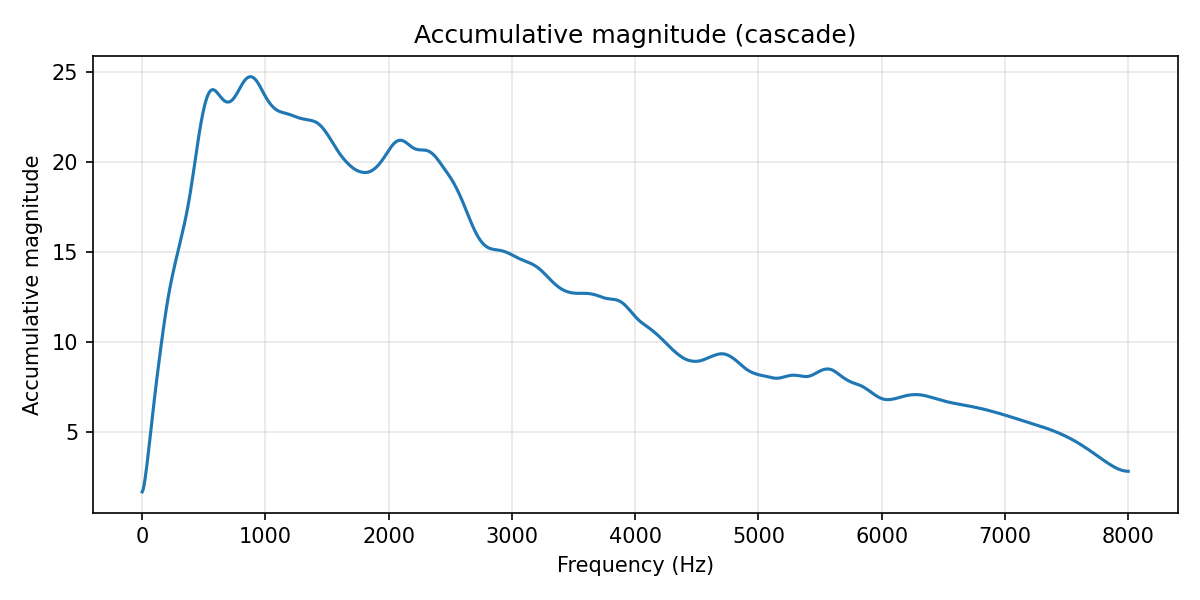
\includegraphics[width=\linewidth]{cascade_accum_mag.png}
  \caption{Accumulative magnitude}
\end{subfigure}\hfill
\begin{subfigure}[t]{0.48\textwidth}
  \centering
  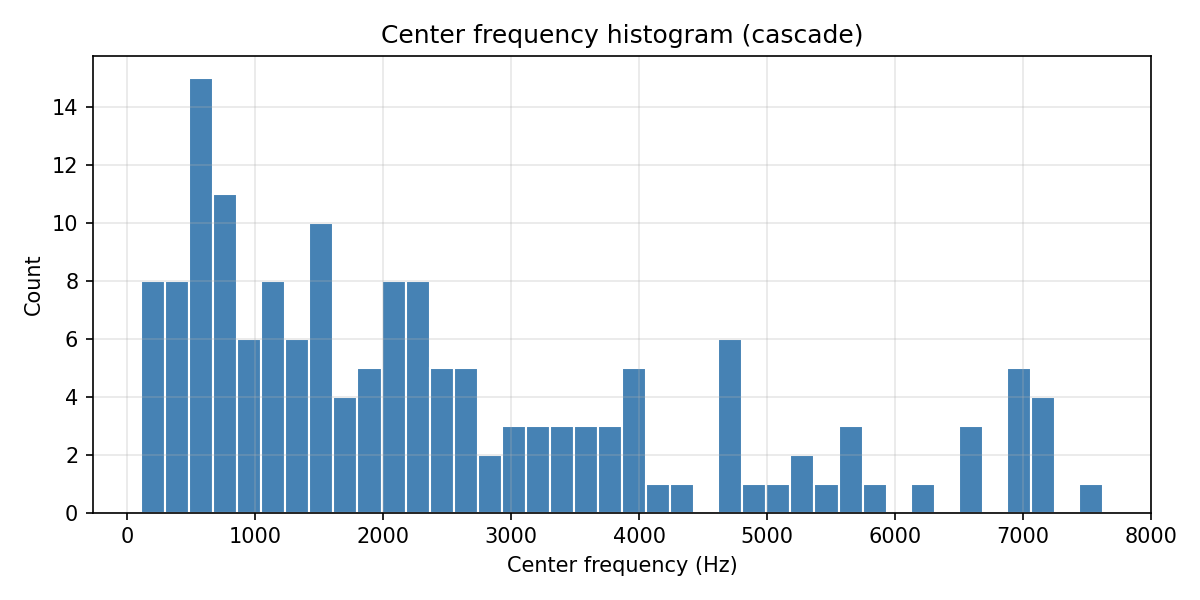
\includegraphics[width=\linewidth]{cascade_fc_hist.png}
  \caption{Center-frequency histogram}
\end{subfigure}
\caption{Cascade filter-bank analysis after TIMIT training.}
\label{fig:cascade-analysis}
\end{figure}

\begin{figure}[H]
\centering
\begin{subfigure}[t]{0.48\textwidth}
  \centering
  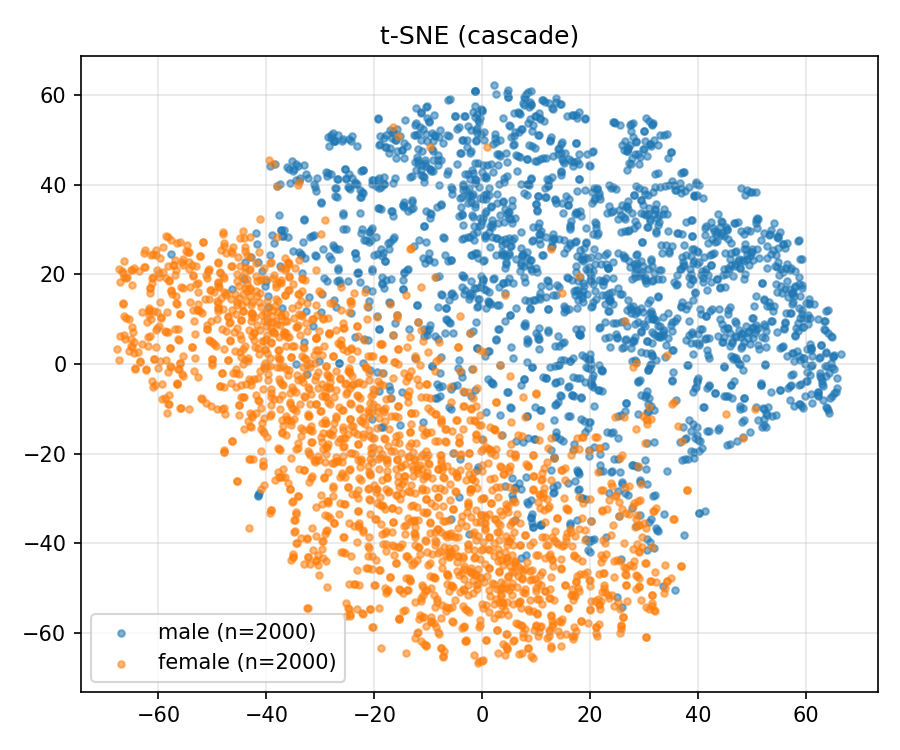
\includegraphics[width=\linewidth]{cascade_tsne.png}
  \caption{t-SNE of Conv features (TIMIT)}
\end{subfigure}\hfill
\begin{subfigure}[t]{0.48\textwidth}
  \centering
  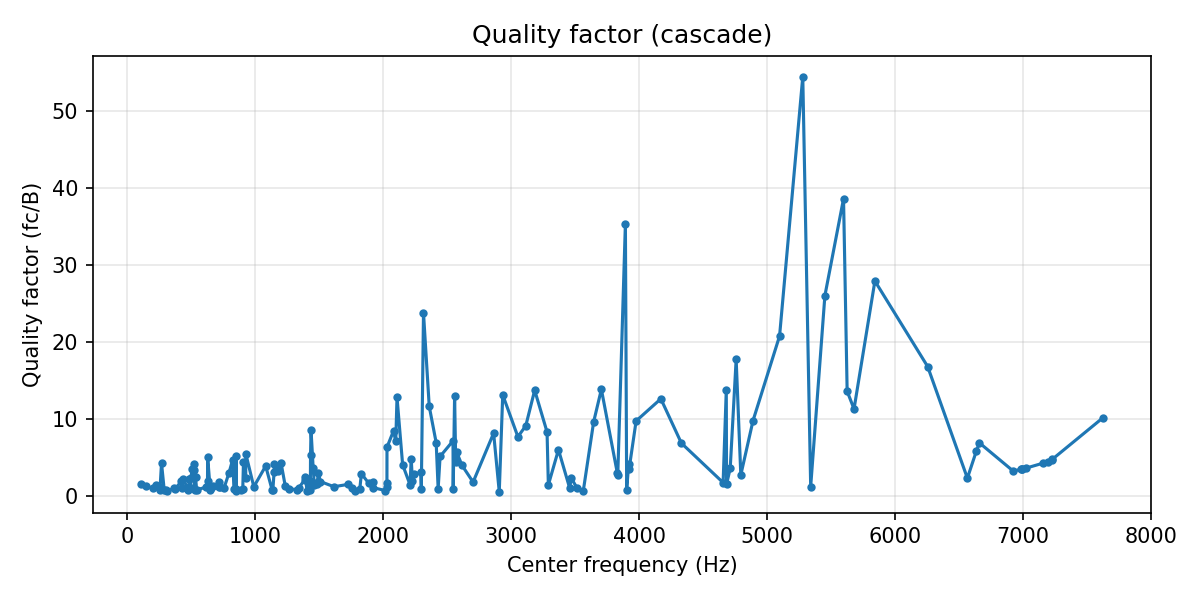
\includegraphics[width=\linewidth]{cascade_qf.png}
  \caption{Quality factor $Q{=}f_c/B$}
\end{subfigure}
\caption{Cascade: feature separability and quality-factor profile.}
\label{fig:cascade-tsne-qf}
\end{figure}

\begin{figure}[H]
\centering
\begin{subfigure}[t]{0.48\textwidth}
  \centering
  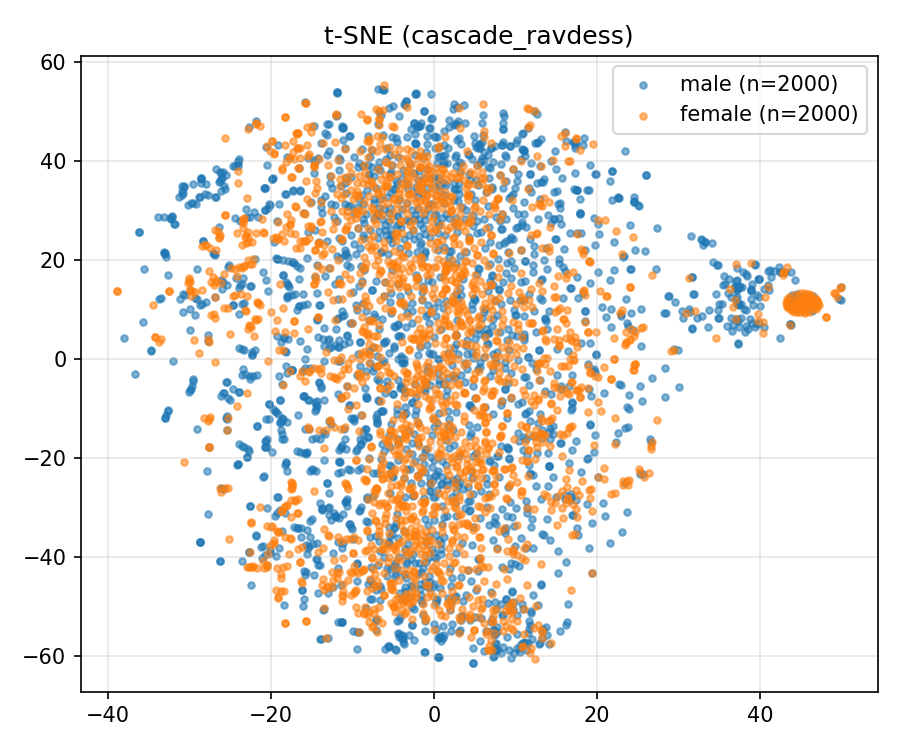
\includegraphics[width=\linewidth]{tsne_cascade_ravdess.png}
  \caption{Cascade after FT (RAVDESS)}
\end{subfigure}\hfill
\begin{subfigure}[t]{0.48\textwidth}
  \centering
  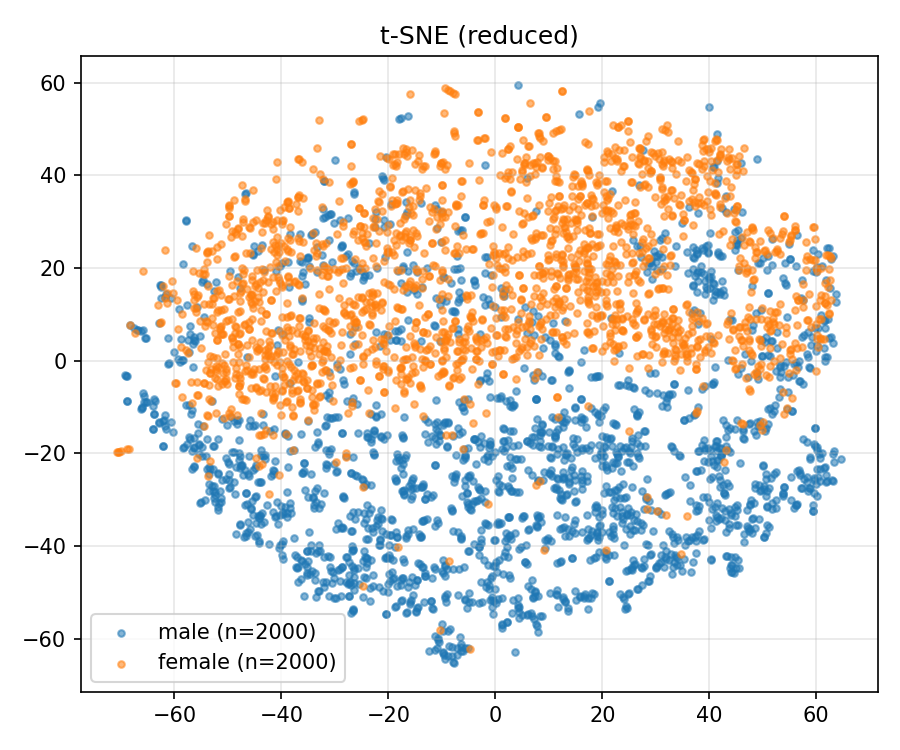
\includegraphics[width=\linewidth]{reduced_tsne.png}
  \caption{Paper Reduced (TIMIT)}
\end{subfigure}
\caption{Domain-shift and Reduced embeddings. Male/female remain separable; Reduced margins are softer (higher FER).}
\label{fig:tsne-extra}
\end{figure}

\begin{figure}[H]
\centering
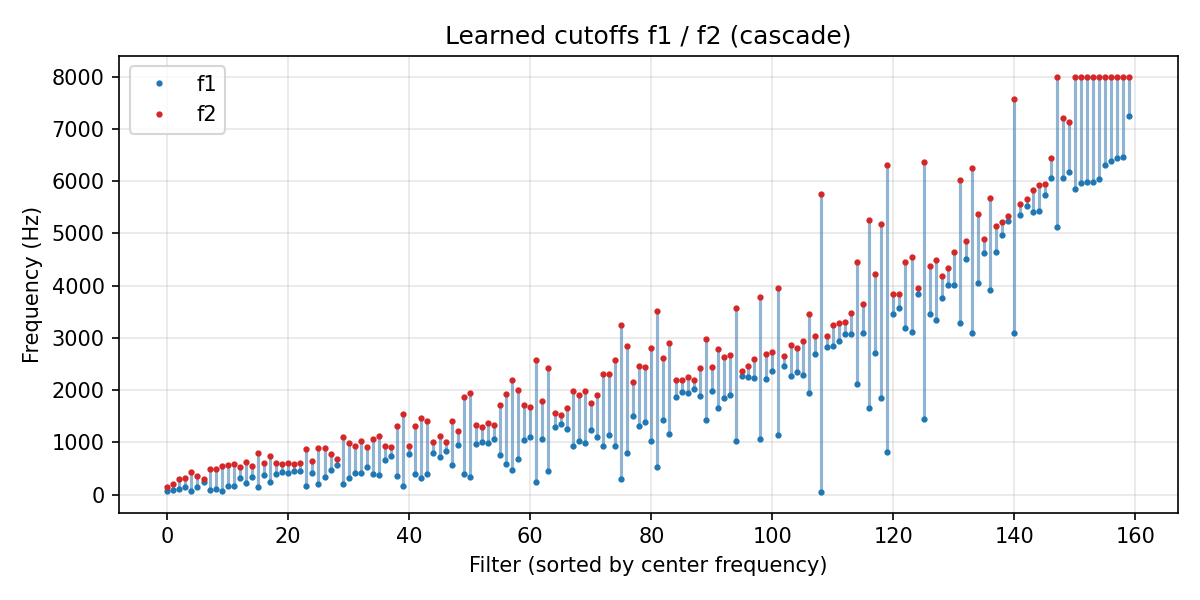
\includegraphics[width=0.92\textwidth]{f1_f2_cascade.png}
\caption{Learned Cascade cutoffs $(f_1,f_2)$ for both stages (160 bands) --- input to pole reduction.}
\label{fig:f1f2}
\end{figure}

% ============================================================
\section{Innovation: Alternative Reduced Filter Banks}
\label{sec:innovation}
% ============================================================

\subsection{Motivation}

Paper Mean-shift reduction is task-agnostic, uses a frequency-uniform complex-plane distance, splits each Cascade filter into two poles, and freezes cutoffs. We keep $K{=}43$ for our proposals so comparisons with the paper Reduced bank are fair.

\subsection{Proposed methods}

\begin{table}[H]
\centering
\caption{Proposed Reduced models (all $K{=}43$ sinc$^2$ filters).}
\label{tab:variants}
\begin{tabular}{@{}llp{6.8cm}@{}}
\toprule
\textbf{Method} & \textbf{Selection} & \textbf{Training} \\
\midrule
Task-aware ERB & ERB-warped weighted mean-shift (Taylor attribution + gender Fisher) & Frozen + CE \\
\textbf{Task-aware distilled} & Same selection as task-aware ERB & KD from Cascade + trainable $f_1/f_2$ (proposed) \\
\bottomrule
\end{tabular}
\end{table}

\paragraph{Task-aware ERB clustering.}
Represent poles in ERB-rate space $(u,v)=(\mathrm{ERB}(f_c),\mathrm{ERB}(f_2)-\mathrm{ERB}(f_1))$. Weight each pole by the average of (i)~Taylor score $\mathbb{E}[|a\,\partial L/\partial a|]$ and (ii)~Fisher score of filter log-energy for gender. Weighted Gaussian mean-shift; bandwidth bisected to obtain $K$ clusters. Cluster-mean cutoffs initialise a \textbf{frozen} sinc$^2$ bank; only the CNN body is trained (50 TIMIT epochs, cross-entropy).

\paragraph{Task-aware distilled (proposed).}
Uses the \textbf{same} $K$ filter bands as task-aware ERB, but does \textbf{not} freeze the Reduced cutoffs. A frozen Cascade teacher provides Hinton distillation~\cite{hinton2015}:
$\mathcal{L}=(1-\alpha)\mathrm{CE}+\alpha T^2\mathrm{KL}$ with $\alpha{=}0.5$, $T{=}4$, jointly with label cross-entropy on TIMIT. This recovers capacity lost when the paper freezes slightly mis-centred Mean-shift bands.

\subsection{Quantitative results}

\begin{table}[H]
\centering
\caption{Proposed Reduced models vs.\ Cascade teacher and paper Mean-shift Reduced ($K{=}43$). TIMIT = in-domain test; RAV / Vox = after LibriSpeech fine-tuning (20 epochs).}
\label{tab:innov}
\small
\begin{tabular}{@{}llrrrrrrr@{}}
\toprule
\textbf{Model} & \textbf{\#F} & \textbf{T.Acc} & \textbf{R.Acc} & \textbf{R.CER} & \textbf{R.FER} & \textbf{V.Acc} & \textbf{V.CER} & \textbf{V.FER} \\
\midrule
Cascade (teacher) & 80 & \textbf{99.18} & 95.49 & 4.51 & 26.32 & \textbf{96.80} & 3.20 & 17.44 \\
Paper Reduced (MS) & 43 & 98.07 & 89.58 & 10.42 & 28.88 & 91.53 & 8.47 & 23.17 \\
Task-aware ERB & 43 & 98.29 & 91.25 & 8.75 & 27.90 & 91.83 & 8.17 & 22.49 \\
\textbf{Task-aware distilled} & 43 & 98.88 & \textbf{95.63} & \textbf{4.37} & 26.10 & 93.48 & 6.52 & 20.73 \\
\bottomrule
\end{tabular}
\end{table}

\begin{table}[H]
\centering
\caption{Gains over paper Mean-shift Reduced (percentage points).}
\label{tab:delta}
\begin{tabular}{@{}lrrr@{}}
\toprule
\textbf{Method} & $\boldsymbol{\Delta}$\textbf{TIMIT} & $\boldsymbol{\Delta}$\textbf{RAVDESS} & $\boldsymbol{\Delta}$\textbf{Vox} \\
\midrule
Task-aware ERB & $+0.22$ & $+1.67$ & $+0.30$ \\
\textbf{Task-aware distilled} & $+0.81$ & $\boldsymbol{+6.05}$ & $\boldsymbol{+1.95}$ \\
\bottomrule
\end{tabular}
\end{table}

\begin{figure}[H]
\centering
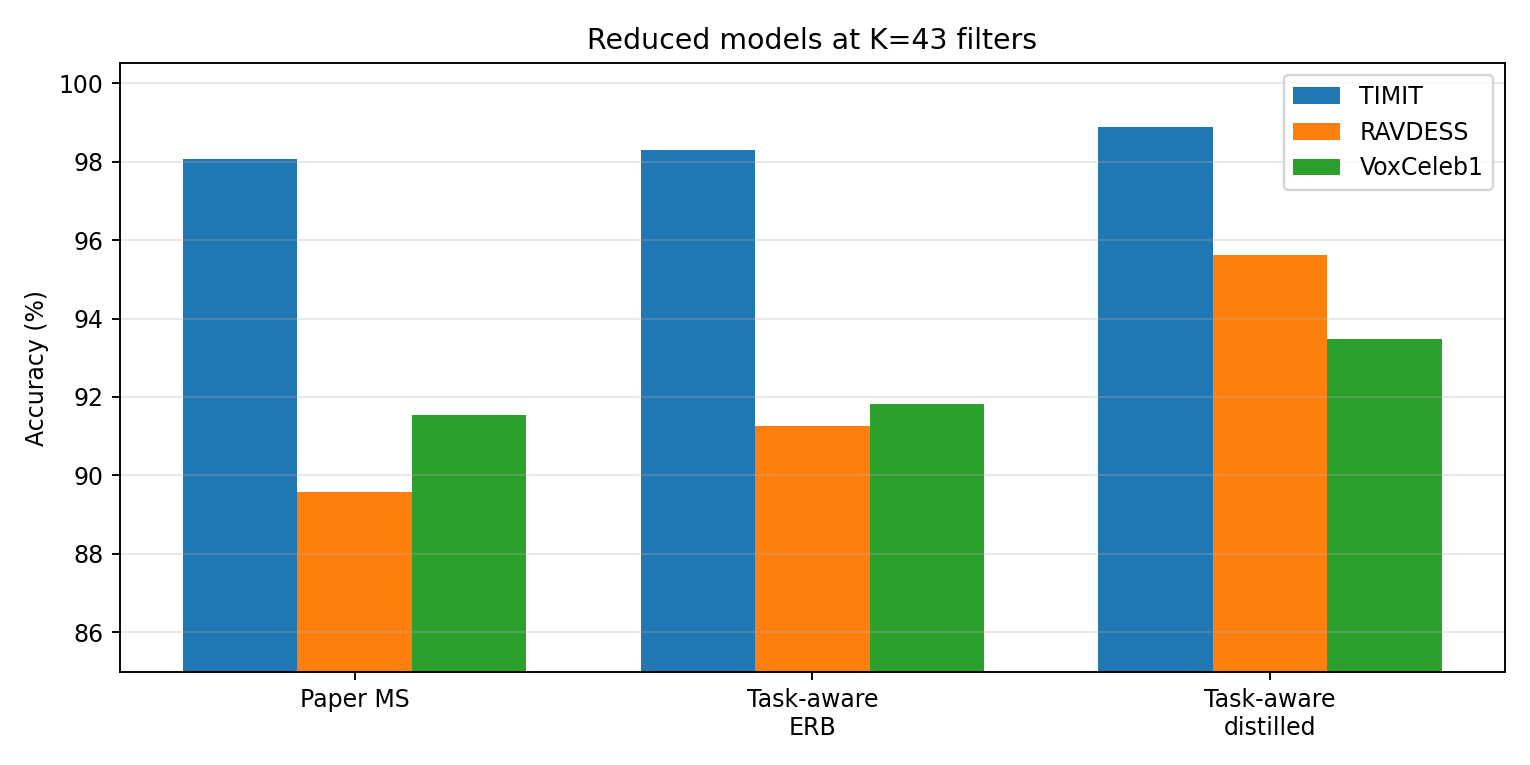
\includegraphics[width=0.98\textwidth]{bar_reduced_variants.png}
\caption{Paper Reduced vs.\ proposed models at equal $K{=}43$ on TIMIT, RAVDESS, and VoxCeleb1-test.}
\label{fig:bar-innov}
\end{figure}

\subsection{Method figures}

\begin{figure}[H]
\centering
\begin{subfigure}[t]{0.48\textwidth}
  \centering
  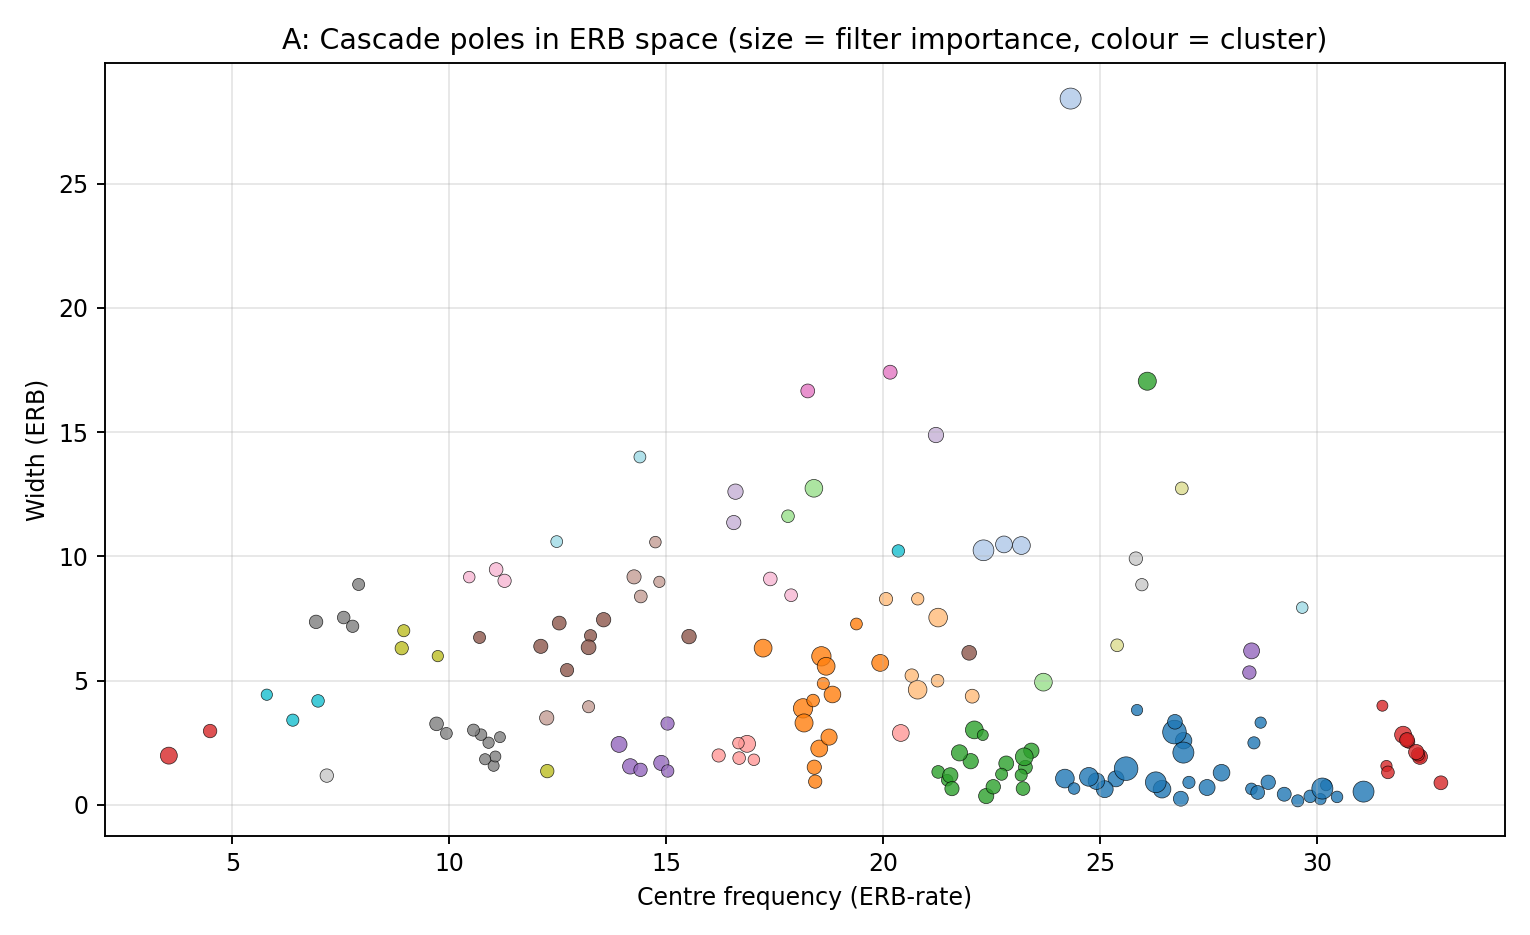
\includegraphics[width=\linewidth]{A_taskaware_erb_clusters.png}
  \caption{Task-aware ERB: poles in ERB space (size $\propto$ importance)}
\end{subfigure}\hfill
\begin{subfigure}[t]{0.48\textwidth}
  \centering
  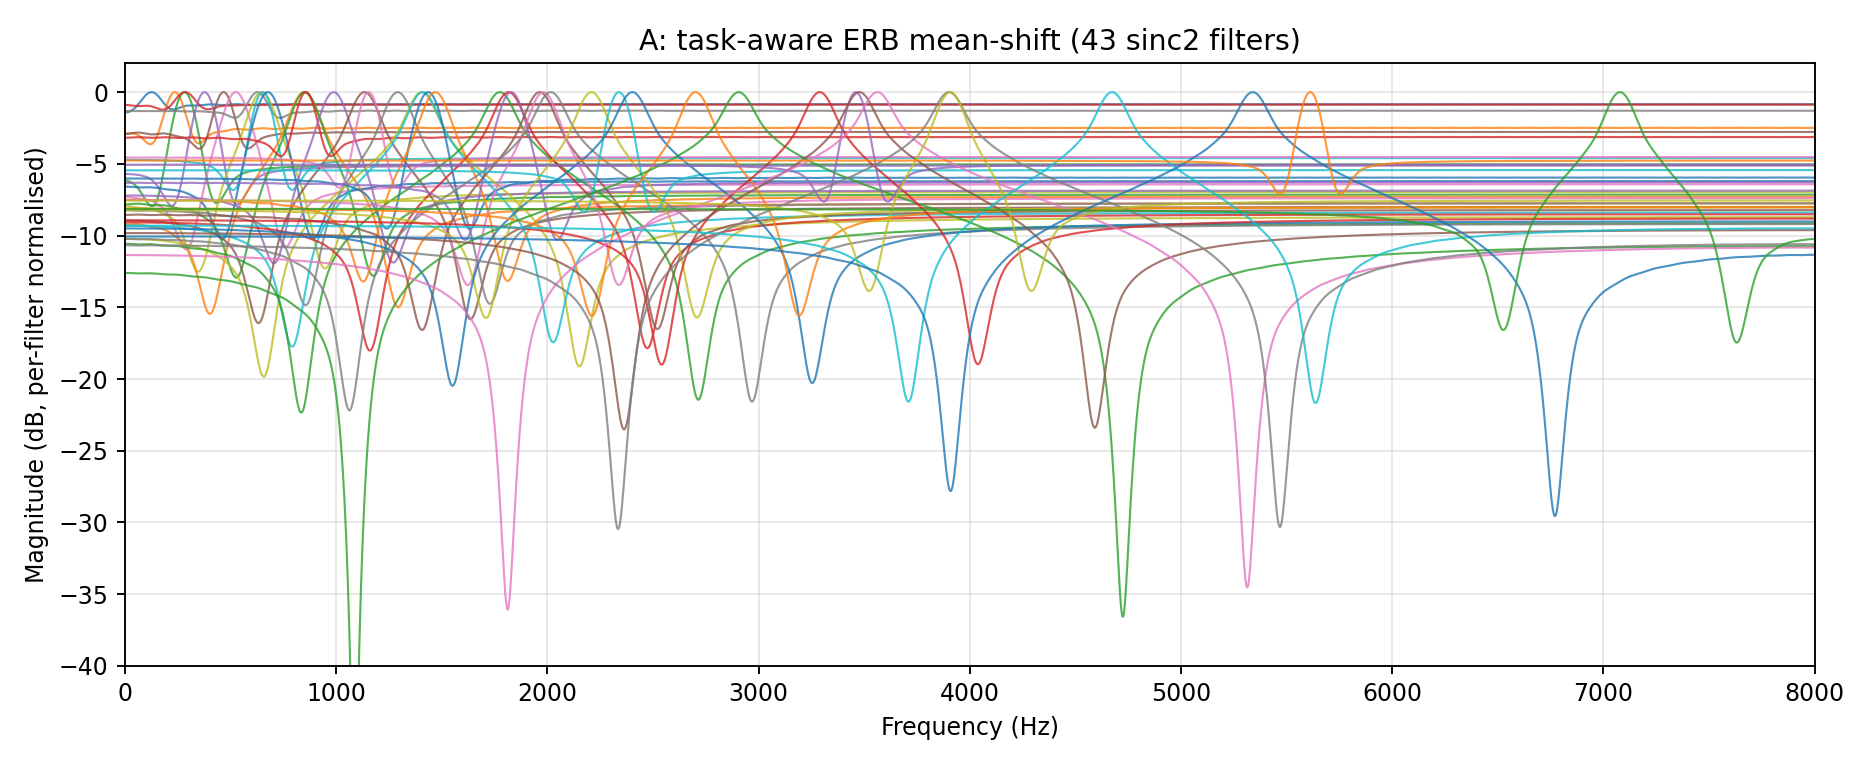
\includegraphics[width=\linewidth]{A_reduced_filter_bank.png}
  \caption{Task-aware ERB: resulting sinc$^2$ bank}
\end{subfigure}
\caption{Task-aware ERB-warped clustering.}
\label{fig:method-a}
\end{figure}

\begin{figure}[H]
\centering
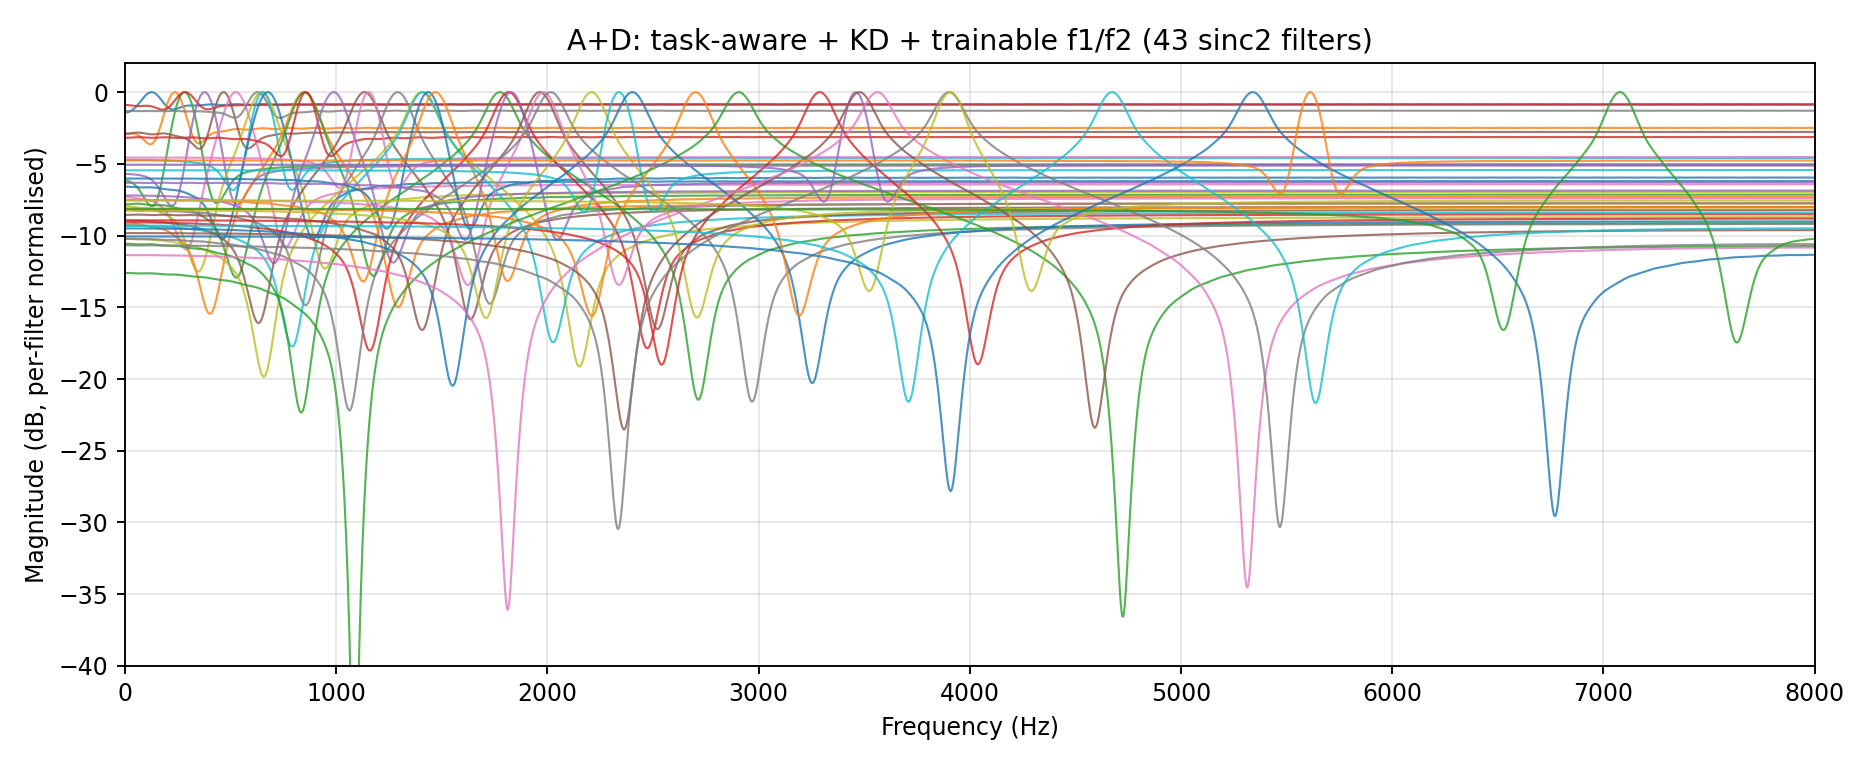
\includegraphics[width=0.72\textwidth]{AD_reduced_filter_bank.png}
\caption{Task-aware distilled: sinc$^2$ filter bank (same band centres as task-aware ERB; cutoffs refined during KD training).}
\label{fig:method-distilled-bank}
\end{figure}

\begin{figure}[H]
\centering
\begin{subfigure}[t]{0.48\textwidth}
  \centering
  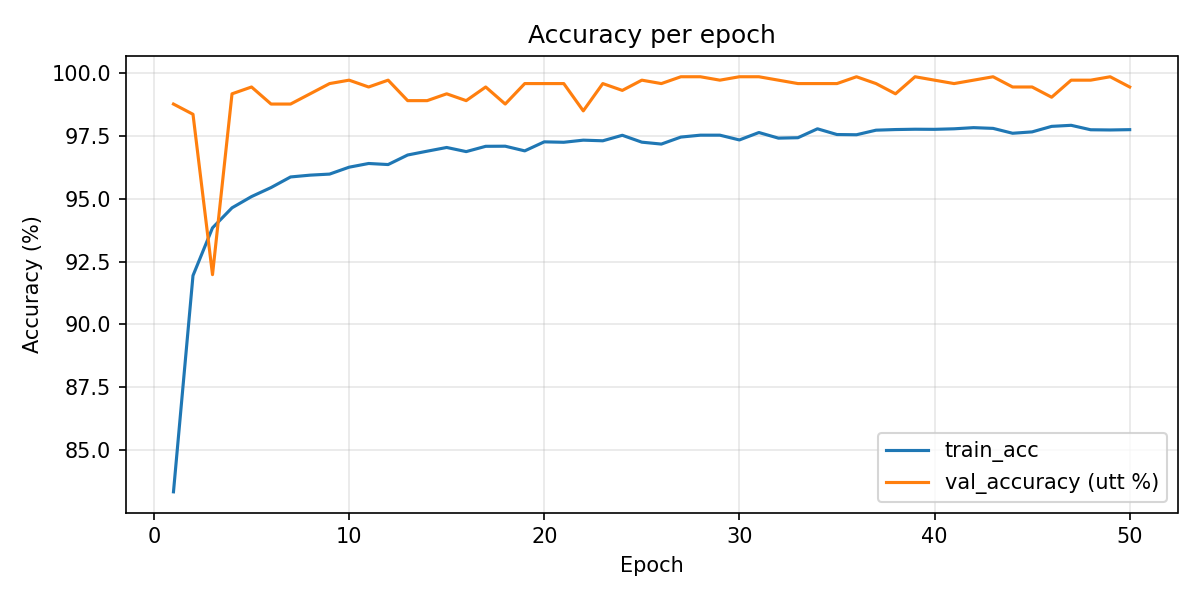
\includegraphics[width=\linewidth]{AD_timit_accuracy.png}
  \caption{Task-aware distilled: TIMIT training}
\end{subfigure}\hfill
\begin{subfigure}[t]{0.48\textwidth}
  \centering
  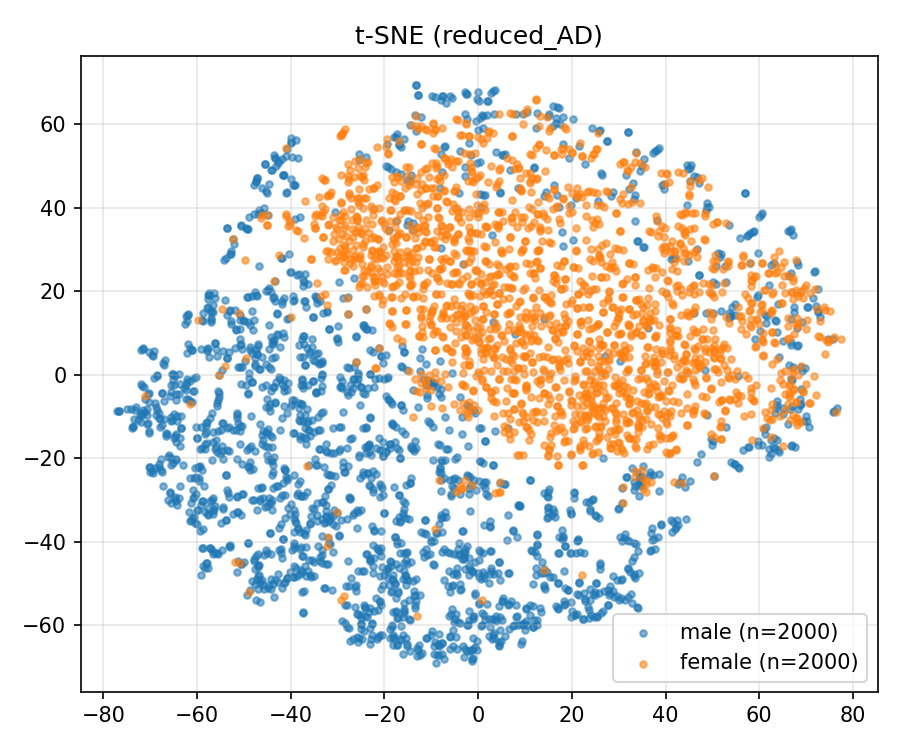
\includegraphics[width=\linewidth]{tsne_reduced_AD.png}
  \caption{Task-aware distilled: t-SNE (TIMIT)}
\end{subfigure}
\caption{Proposed task-aware distilled model: RAVDESS Acc 95.63\% with 43 filters.}
\label{fig:ad-extra}
\end{figure}

\paragraph{Takeaways.}
\begin{itemize}[leftmargin=1.6em,itemsep=0.25em]
  \item \textbf{Task-aware ERB} improves over frozen Mean-shift on all three sets with selection alone ($+0.22$--$+1.67$ pp).
  \item \textbf{Task-aware distilled} adds KD and trainable cutoffs on the same bands and is the best compact model for transfer ($+6.05$ RAVDESS, $+1.95$ Vox vs.\ paper Reduced).
\end{itemize}

% ============================================================
\section{Discussion}
\label{sec:discussion}
% ============================================================

\subsection{Why TIMIT matches}

With SGR\_AFM-aligned kernels and cutoffs, 50 epochs suffice for near-ceiling in-domain Acc. Cascade matches Table~4 almost exactly.

\subsection{Why OOD still lags the paper (for some cells)}

\begin{enumerate}[leftmargin=1.6em,itemsep=0.25em]
  \item Fine-tune 20 vs.\ 200 epochs;
  \item \texttt{dev-clean} vs.\ \texttt{train-clean-360};
  \item VoxCeleb1-test only;
  \item Single seed vs.\ mean of three runs.
\end{enumerate}
Despite this, Sinc/Cascade remain close on Vox, and Gauss exceeds the paper mean on RAVDESS in this run.

\subsection{Reduced story}

Paper Mean-shift Reduced ($K{=}43$) is compact but loses OOD Acc under our budget. \textbf{Task-aware distilled} recovers most of that gap and even slightly exceeds Cascade on RAVDESS in this single run (95.63\% vs.\ 95.49\%) while using roughly half the filters.

% ============================================================
\section{Conclusions}
% ============================================================

\begin{enumerate}[leftmargin=1.6em,itemsep=0.3em]
  \item The reproduction pipeline faithfully matches in-domain AFM ranking; Cascade is best on TIMIT (99.18\%).
  \item Best transfer AFM: Sinc on VoxCeleb1-test (96.96\%).
  \item Paper Mean-shift Reduced (43 frozen filters) is a solid compact baseline but weaker OOD here.
  \item \textbf{Task-aware ERB} gives modest gains with frozen bands; \textbf{task-aware distilled} (same selection + KD + trainable cutoffs) is the best Reduced model for transfer (+6.05 RAVDESS, +1.95 Vox vs.\ paper Reduced at equal $K$).
\end{enumerate}

\begin{thebibliography}{9}
\bibitem{fayyazi2023}
H.~Fayyazi and Y.~Shekofteh,
\textit{Exploiting auditory filter models as interpretable convolutional frontends to obtain optimal architectures for speaker gender recognition},
Applied Acoustics, vol.~213, art.~109635, 2023.

\bibitem{hinton2015}
G.~Hinton, O.~Vinyals, and J.~Dean,
\textit{Distilling the Knowledge in a Neural Network},
arXiv:1503.02531, 2015.

\bibitem{ravanelli2018}
M.~Ravanelli and Y.~Bengio,
\textit{Speaker Recognition from Raw Waveform with SincNet},
SLT, 2018.
\end{thebibliography}

\end{document}
